\section{The Spectrum of Sound}

Sound is a vibration of some body transmitted through the air and perceived by your ears. If you move up and down your hand once per second, we say that your hand vibrates at a frequency of 1 Hertz (Hz). If you move it up and down twice per second, the frequency is 2 Hz. If you could do it about 20 times per second (20 Hz), your eardrums would start sensing the vibration transmitted through the air. Probably you can do it with your hand, but you can use a string on a guitar, the membrane of a drum, the air inside a flute, your vocal folds, the body of a bell... Typically a human can hear vibrations with a frequency between 20 and 20 000 Hz. The higher the frequency, the higher the pitch of the sound.

However, if you use a guitar string or a flute as vibrating bodies, the sound you will perceive will be very different in each of the two cases. This is because we almost never hear a ``pure'' frequency, any natural sound is a mixture of vibrations at different frequencies and varying intensities. A guitar string tuned at a middle A note, will vibrate at 440 Hz. This is the fundamental frequency, but the string will inevitably vibrate also at 880 Hz (the double), 1320 Hz (the triple), and with all the multiple frequencies (called harmonic frequencies), but with less intensity each time. A flute will also vibrate at all these frequencies, but with different intensities. It is the varying intensities of the harmonic frequencies that makes our ear distinguish between guitar and flute. The set of frequencies with their intensities is called the spectrum of the sound, and it defines what we call timbre in music.

What would be a ``pure'' sound, just one frequency and no ``contamination'' from others? Mathematically, we can describe this sound as a sinusoidal wave. It is the sound that would make a perfectly elastic spring that could vibrate without losing any energy. We can't build such a spring, but we can make the membrane of a speaker vibrate at this pure frequency using electronics. A surprising, yet totally useful result in mathematics, is that every periodic function of period $2\pi$ can be approximated by summing up a sequence of sine waves if they are scaled and shifted appropriately. In a formula: 
$$g(t) \approx A_0 + \sum_{i=1}^N A_i \cdot \sin(i t + \varphi_i).$$


This implies that by adding appropriate sine waves we can simulate any static sound, the only information needed is the set of intensities $A_i$ and the phase shifts $\varphi_i$. This has deep implications. On the one hand it allows us to decompose of a complex signal into many simpler ones in a very structured way. Thus, it makes things much simpler to analyze and understand. On a more abstract level it connects different spaces: the time space where signals are described by values (like air pressure) changing over time and the frequency space where signals are composed from simpler ones. Depending on the situation it might be way easier to address a certain problem in one space or the other.

Its applications are far reaching and cover many diverse areas besides sound and music, such as communication technology, quantum theory, coding theory, statistics, electrical circuit design, and an endless series of other topics.

\begin{wrapfigure}{l}{0.35\textwidth}
\centering
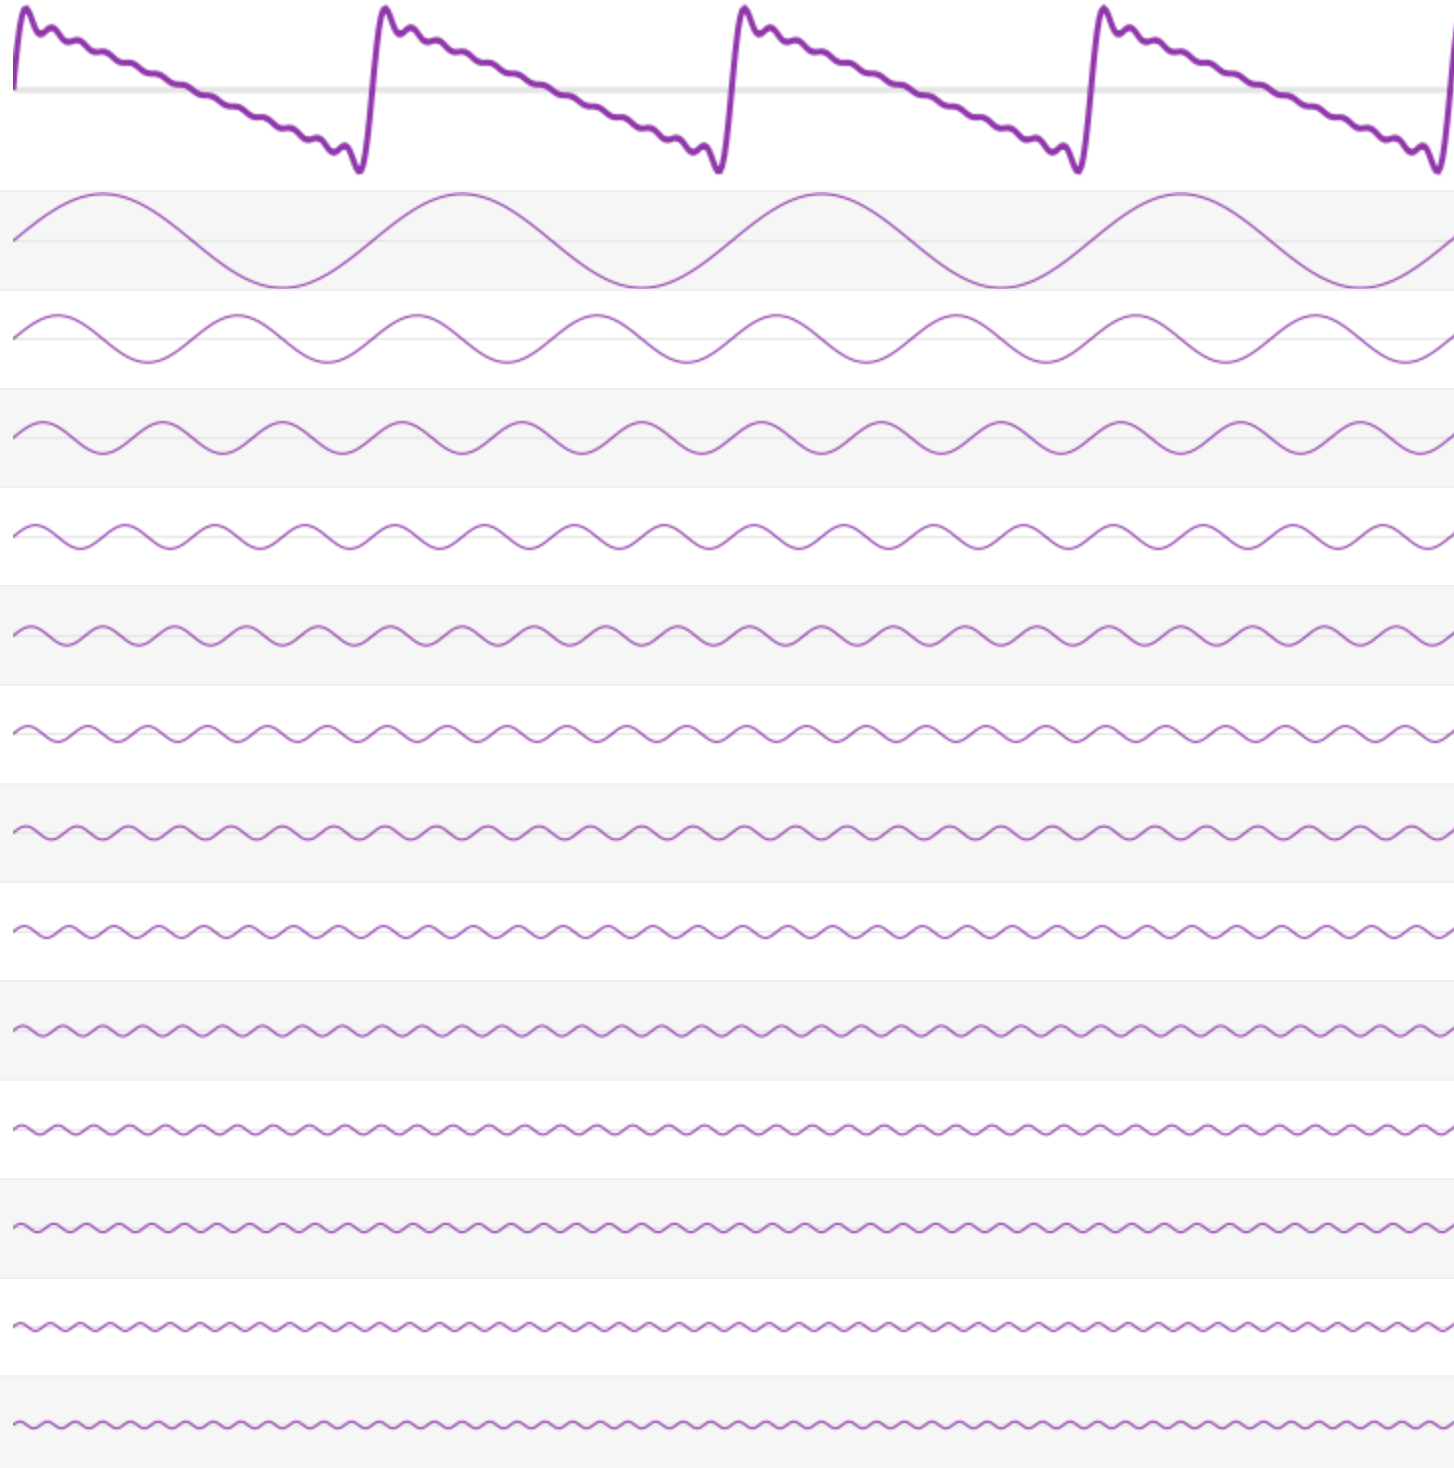
\includegraphics[width=0.35\textwidth]{SpectrumOfSound_1}
\caption*{A sawtooth wave as a sum of sine waves.}
\end{wrapfigure}
On the first screen of the exhibit, you can try to generate a wave by adding harmonic frequencies. Use just one frequency (sine) to hear a ``mathematically pure'' sound. Adjust the intensity of each of the harmonic frequencies, or click on the square or sawtooth waves, to hear different timbres. 

Heuristically, a string instrument has more intense harmonics, and wind instruments have less intense harmonics. But anyway, we are still far from a full synthesizer. To simulate a real instrument, we have to take into account that the sound is not static and eternal, it starts at some point, increases in intensity, then it decays and fades out. So, frequencies and their intensities change through time. Instruments such as bells, xylophones and most percussions do not have a spectrum formed by multiples of a fundamental frequency, but other frequencies depending on the geometric shape of the vibrating body. Therefore, it is quite difficult to synthesize a real instrument.

However, there is an extraordinary mathematical tool that allows us to reverse the process. Instead of adding up frequencies to obtain a composed signal, the Fourier transform is a procedure that allows to take an arbitrary signal (recorded with a microphone, for instance) and to decompose it into its fundamental pieces: the frequencies and their intensities that you would need to use to generate the signal using pure frequencies as building blocks. 

Let $g(t)$ be a signal represented as a function, so that for each time t it returns the intensity of the sound (this intensity may be the air pressure, or the voltage in the line wire of a microphone). The Fourier transform of a signal $g(t)$ is a new function $\hat g(t)$ that for each frequency $f$ returns the intensity of a sine wave with that frequency required to synthesize the signal $g(t)$. It is achieved with this formula:
$$\hat g(f) = \int_{-\infty}^{\infty} g(t)\ e^{2\pi i f t } \ dt$$

Note that there are complex values inside the integral, so that the Fourier transform is a complex-valued function. This is because there are two pieces of information needed to synthesize a signal: the amplitude $A_i$ and the phase shifts $\varphi_i$. 

The Fourier transform gives both the amplitude and phase of the signal as modulus and argument of the complex value. Usually, for audio analysis often only the modulus is used to obtain a graph with peaks at the most prominent frequencies, which is sufficient to reconstruct the original signal with accuracy.

\begin{wrapfigure}{r}{0.45\textwidth}
\centering
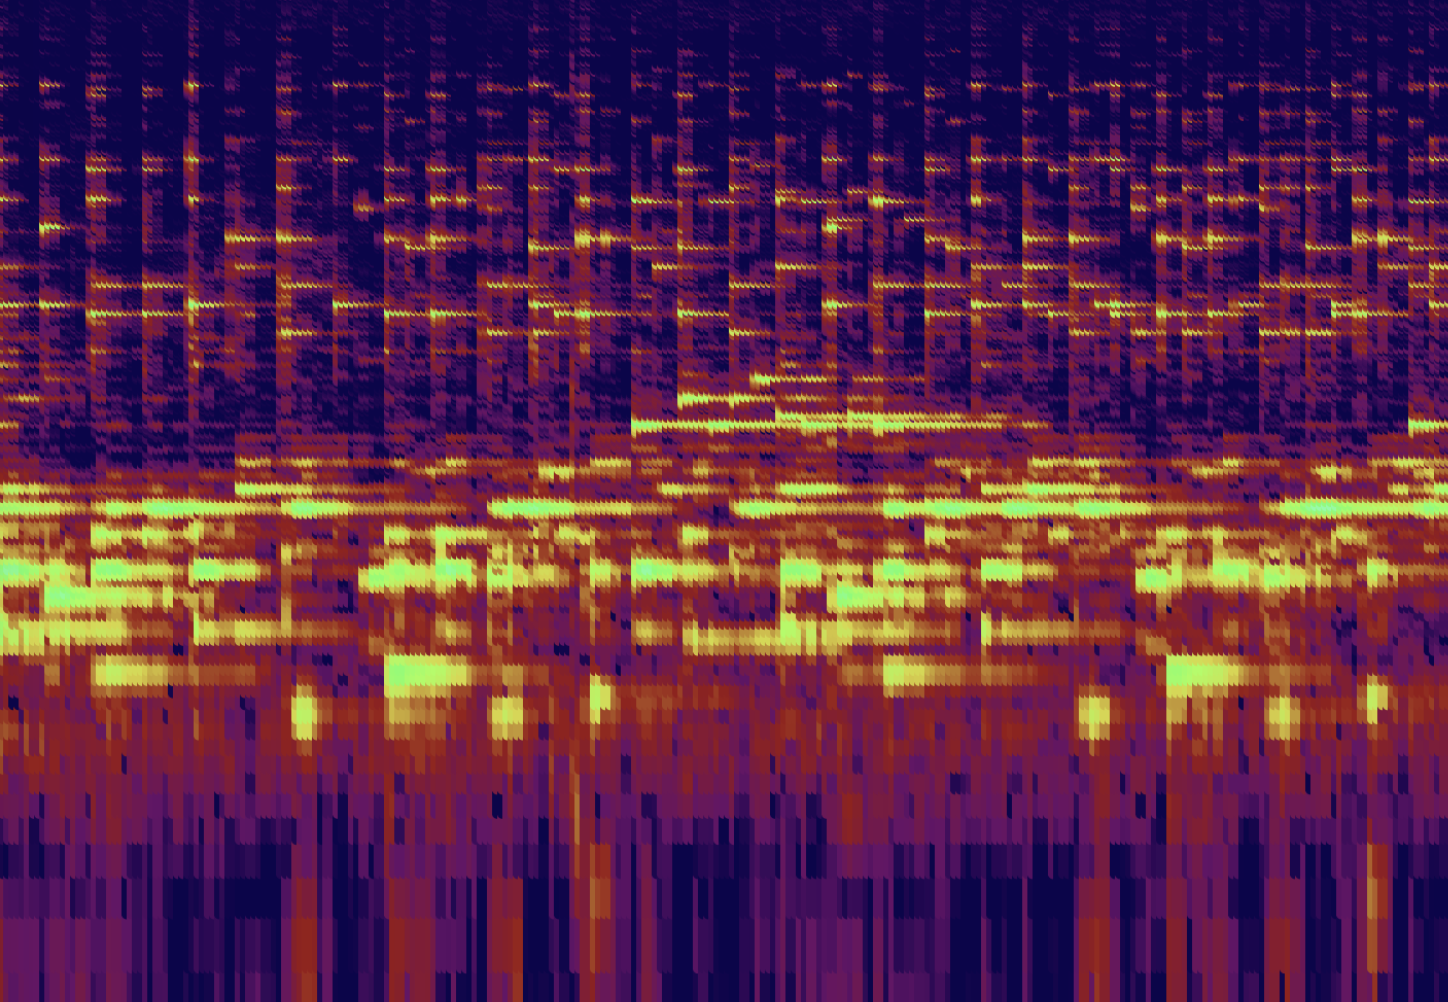
\includegraphics[width=0.45\textwidth]{SpectrumOfSound_2}
\caption*{Sonogram of part of Pachelbel's canon.}
\end{wrapfigure}

For practical applications, there is a useful algorithm called the Fast Fourier Transform (FFT), that substitutes the abstract mathematical formula. This allows us to make extremely fast computations and analyze signals in real time. Today many electronic ways of working with music are based on FFT. It forms the first step of extracting a score from a piece of played music. It can be used for instance for the automatic transcription of Jazz soli. It is also the basis of modifying music. The common practice of pitch adjustment in pop music (auto-tune) can be basically described as an ``analyze - correct - synthesis'' procedure. Special sound effects like letting an instrument speak like a human voice rely on automatic sound analysis of the involved spectra. Also automatic music recognition services like Shazam heavily rely on the fingerprint of a tune resembled by its sonogram.

The second screen of the exhibit displays a spectrum analyzer connected to the microphone input. On the left you have the spectrum, i.e. the instantaneous analysis of frequencies (Fourier transform) of the playing signal. At the right the spectrum leaves a trace to visualize the history of the input signal (sonogram). 

\begin{figure}[h]
\centering
\begin{subfigure}{0.45\textwidth}
\centering
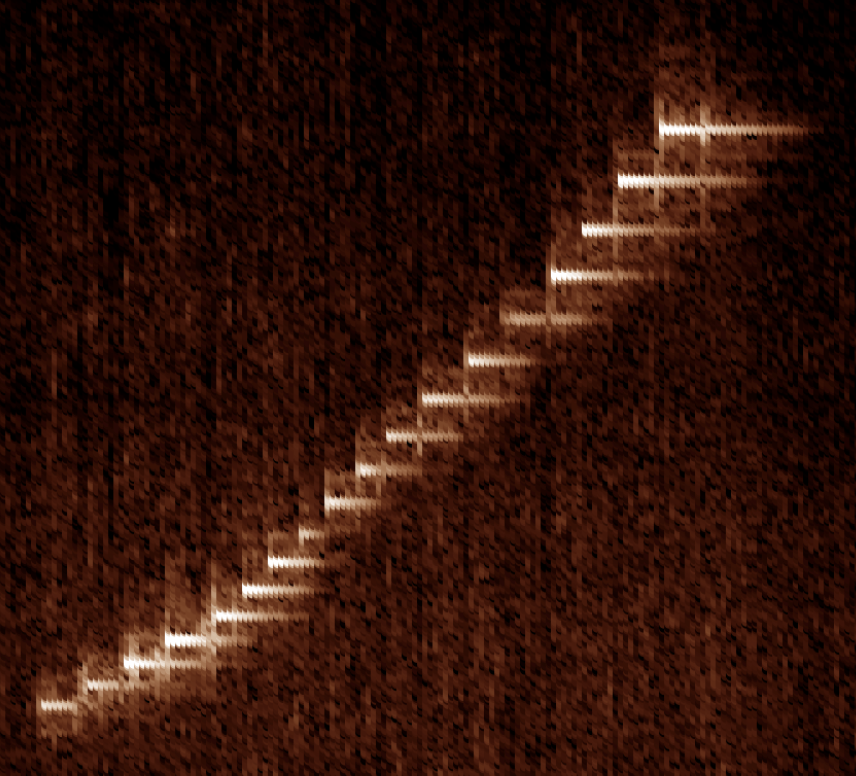
\includegraphics[height=3cm]{SpectrumOfSound_7}
\subcaption*{Chromatic scale linear.}
\end{subfigure}
\begin{subfigure}{0.45\textwidth}
\centering
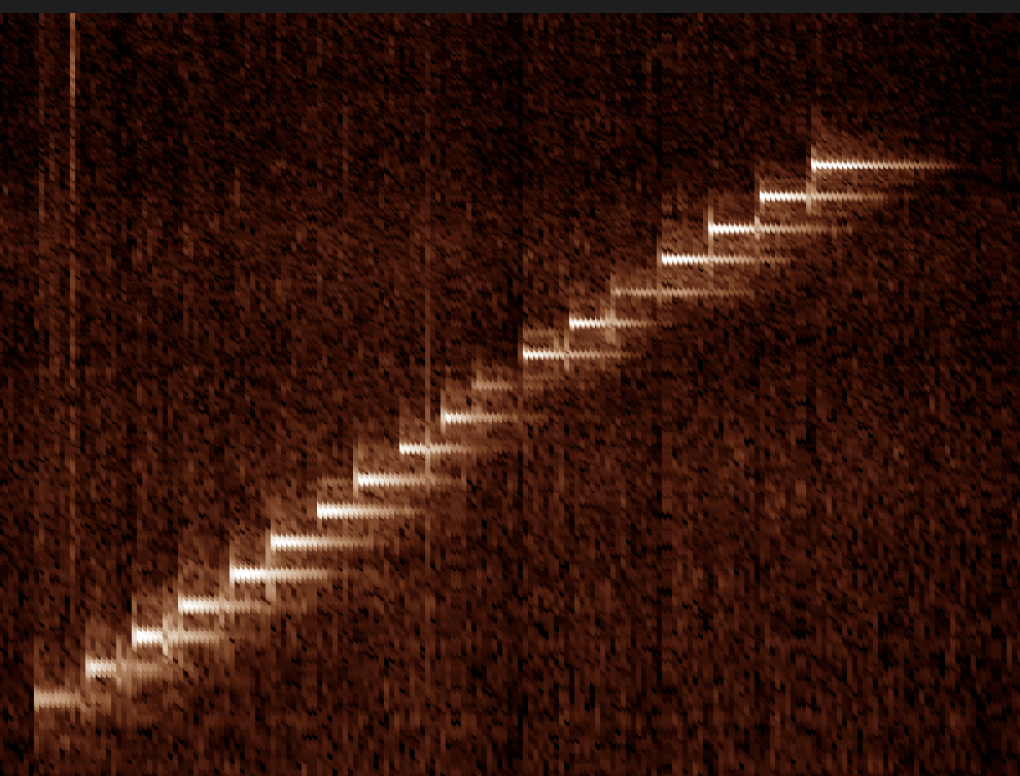
\includegraphics[height=3cm]{SpectrumOfSound_8}
\subcaption*{Chromatic scale logarithmic.}
\end{subfigure}
\end{figure}

Linear scale is best suited for sounds and overtones (frequencies $f$, $2f$, $3f$, $4f$, $5f$, ...), while logarithmic scale is best suited for musical tones (frequencies $f$, $af$, $a^2 f$, $a^2 f$, $a^2 f$, ...). Use the microphone to analyze your voice or the available instruments. Sing something, make noises, talk, or use the synthesizer to generate a tone. Put the microphone next to the speaker and analyze the sound produced. Try to identify the frequencies, their intensities, when they appear, when they fade out.


\begin{figure}[h]
\centering
\begin{subfigure}{0.45\textwidth}
\centering
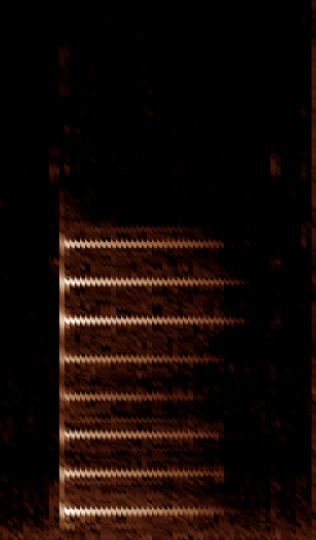
\includegraphics[height=3cm]{SpectrumOfSound_5}
\caption*{Overtones linear.}
\end{subfigure}
\begin{subfigure}{0.45\textwidth}
\centering
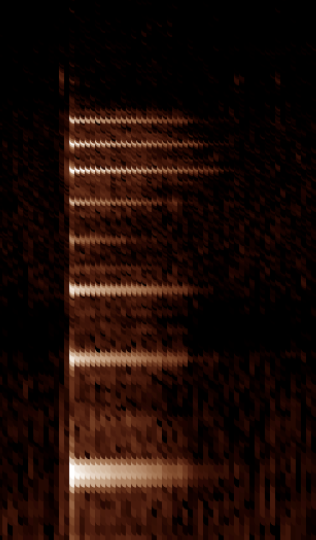
\includegraphics[height=3cm]{SpectrumOfSound_6}
\caption*{Overtones logarithmic.}
\end{subfigure}
\end{figure}


\vfill

Authors of this exhibit: \\ 
Synthesiser: Tero Parviainen, Eric Londaits (IMAGINARY). \\
Analyser: Jürgen Richter-Gebert (TU Munich). \\
Text: Daniel Ramos (IMAGINARY).

